%%\documentclass[a4paper,11pt]{article}
\documentclass[11pt]{article}

\usepackage[left=2.5cm, right=2cm, top=0.6cm, bottom=2cm, includehead, includefoot]{geometry}
\usepackage[utf8]{inputenc}
\usepackage[T1]{fontenc}
\usepackage{titlesec}
\usepackage{enumitem}
\usepackage{graphicx}
\usepackage{amsmath}
\usepackage{amsfonts}
\usepackage{amssymb}
\usepackage{parskip}
\usepackage{float}
\usepackage{setspace}
\usepackage{fancyhdr}
\usepackage{needspace}
\usepackage{etoolbox}

\pagestyle{fancy}
\fancyhf{}
\setlength{\headheight}{63pt}
\setlength{\headsep}{10pt}
\fancyhead[L]{}
\fancyhead[R]{}
\fancyhead[C]{\includegraphics[width=\textwidth]{picture/logo.pdf}}
\renewcommand{\headrulewidth}{0pt}
\fancyfoot[C]{\thepage}
\setlength{\footskip}{18pt}

\setstretch{1.12}
\setlength{\parskip}{0.65em}
\setlist[itemize]{leftmargin=1.35cm, itemsep=0.45em, topsep=0.35em}
\setlist[enumerate]{leftmargin=1.35cm, itemsep=0.45em, topsep=0.35em}

\titleformat{\section}{\normalfont\Large\bfseries}{\thesection}{1em}{}
\titleformat{\subsection}{\normalfont\large\bfseries}{\thesubsection}{1em}{}
\preto{\subsection}{\Needspace{10\baselineskip}}
\preto{\subsubsection}{\Needspace{8\baselineskip}}

\title{Informe del Proyecto}
\raggedbottom

\begin{document}

\renewcommand{\figurename}{Figura}
\renewcommand{\thesection}{\Roman{section}}
\begin{center}
    \textbf{\underline{\normalsize APE 1}}
\end{center}

\section{PORTADA}

\begin{tabbing}
    \textbf{Unidad de Organización Curricular:}\hspace{1cm} \= \kill
    \textbf{Tema:} \> Procesamiento de Imágenes en Dominio Espacial y Frecuencia \\[0.25em]
    \textbf{Carrera:} \> Ingeniería de Software \\[0.25em]
    \textbf{Unidad de Organización Curricular:} \> PROFESIONAL \\[0.25em]
    \textbf{Nivel y Paralelo:} \> Séptimo A \\[0.25em]
    \textbf{Alumnos participantes:} \> Paul Velastegui \\
    \> David Manjarres \\[0.25em]
    \textbf{Asignatura:} \> Inteligencia Artificial \\[0.25em]
    \textbf{Docente:} \> Ing. Rubén Nogales, Mg.
\end{tabbing}

\section{INFORME DE GUÍA PRÁCTICA}
\renewcommand{\thesection}{\arabic{section}}

\subsection{Objetivos}
\textbf{General:}
\begin{itemize}
    \item Desarrollar una aplicación de escritorio para procesar imágenes digitales mediante una cadena de preprocesamiento y una comparación entre filtros del dominio espacial y del dominio de frecuencia.
\end{itemize}

\textbf{Específicos:}
\begin{itemize}
    \item Implementar manualmente la conversión a escala de grises, la ecualización del histograma, la binarización y los filtros espaciales de media, mediana y moda.
    \item Aplicar ruido sal y pimienta sobre una imagen binarizada para evaluar la respuesta de los filtros espaciales.
    \item Aplicar un filtro gaussiano pasa bajas en el dominio de frecuencia usando FFT y analizar su efecto mediante el espectro, la máscara y la reconstrucción final.
\end{itemize}

\subsection{Modalidad}
\begin{tabbing}
    \hspace{1cm} \= Presencial.
\end{tabbing}

\subsection{Tiempo de duración}
\begin{tabbing}
    \hspace{1cm} \= \textbf{Presenciales:} \= 8 \\
    \hspace{1cm} \= \textbf{No presenciales:} \= 0
\end{tabbing}

\subsection{Instrucciones}
\begin{enumerate}
    \item Seleccionar una imagen de entrada para realizar el procesamiento.
    \item Convertir la imagen a escala de grises y aplicar ecualización del histograma.
    \item Ajustar el umbral de binarización y la cantidad de ruido sal y pimienta.
    \item Comparar los resultados de los filtros espaciales media, mediana y moda.
    \item Evaluar el filtrado gaussiano en frecuencia modificando el parámetro $D_0$.
\end{enumerate}

\subsection{Listado de equipos, materiales y recursos}
Listado de equipos y materiales generales empleados en la guía práctica:
\begin{itemize}
    \item Computador.
    \item Imagen de prueba en formato común (\texttt{png}, \texttt{jpg}, \texttt{jpeg} o \texttt{bmp}).
    \item Entorno de desarrollo Python 3.
    \item Herramientas que permitan generar documentos en formato PDF.
\end{itemize}

\subsubsection*{Dependencias de Python utilizadas}
También se emplearon las siguientes librerías:
\begin{itemize}
    \item \textbf{OpenCV (\texttt{opencv-python}):} Utilizada para cargar la imagen desde disco y convertirla de BGR a RGB.
    \item \textbf{NumPy (\texttt{numpy}):} Utilizada como estructura matricial para la imagen y para la transformada rápida de Fourier.
    \item \textbf{PySide6 (\texttt{PySide6}):} Framework usado para construir la interfaz gráfica de escritorio.
    \item \textbf{Matplotlib (\texttt{matplotlib}):} Utilizada para mostrar imágenes e histogramas dentro de la interfaz.
\end{itemize}

\textbf{TAC (Tecnologías para el Aprendizaje y Conocimiento) empleados en la guía práctica:}

$\square$ Plataformas educativas \\
$\square$ Simuladores y laboratorios virtuales \\
$\blacksquare$ Aplicaciones educativas \\
$\square$ Recursos audiovisuales \\
$\square$ Gamificación \\
$\blacksquare$ Inteligencia Artificial \\
Otros (Especifique): \underline{\hspace{5cm}}

\subsection{Actividades por desarrollar}
\begin{enumerate}
    \item Cargar una imagen RGB y obtener su versión en escala de grises.
    \item Ecualizar el histograma de la imagen en grises y binarizarla con un umbral ajustable.
    \item Inyectar ruido sal y pimienta para generar una base de prueba común.
    \item Aplicar filtros espaciales y comparar su resultado con el filtrado gaussiano en frecuencia.
\end{enumerate}

\subsection{Fundamentación y Selección del Caso de Estudio}

La herramienta se diseñó para estudiar dos enfoques de procesamiento de imágenes: el dominio espacial y el dominio de frecuencia. En el dominio espacial la operación se realiza directamente sobre los valores de los píxeles y sus vecinos. En el dominio de frecuencia la imagen se transforma primero a una representación espectral, donde es posible separar componentes de baja y alta frecuencia.

\subsubsection{Caso de prueba}

Para validar la aplicación se empleó una imagen de prueba con suficiente variación de intensidades y textura, de manera que fuera posible observar con claridad el efecto de la ecualización, la binarización, el ruido impulsivo y los filtros posteriores. La herramienta permite trabajar con cualquier imagen común cargada por el usuario, por lo que el caso de estudio puede cambiar sin alterar el flujo del algoritmo.

\begin{figure}[!htbp]
    \centering
    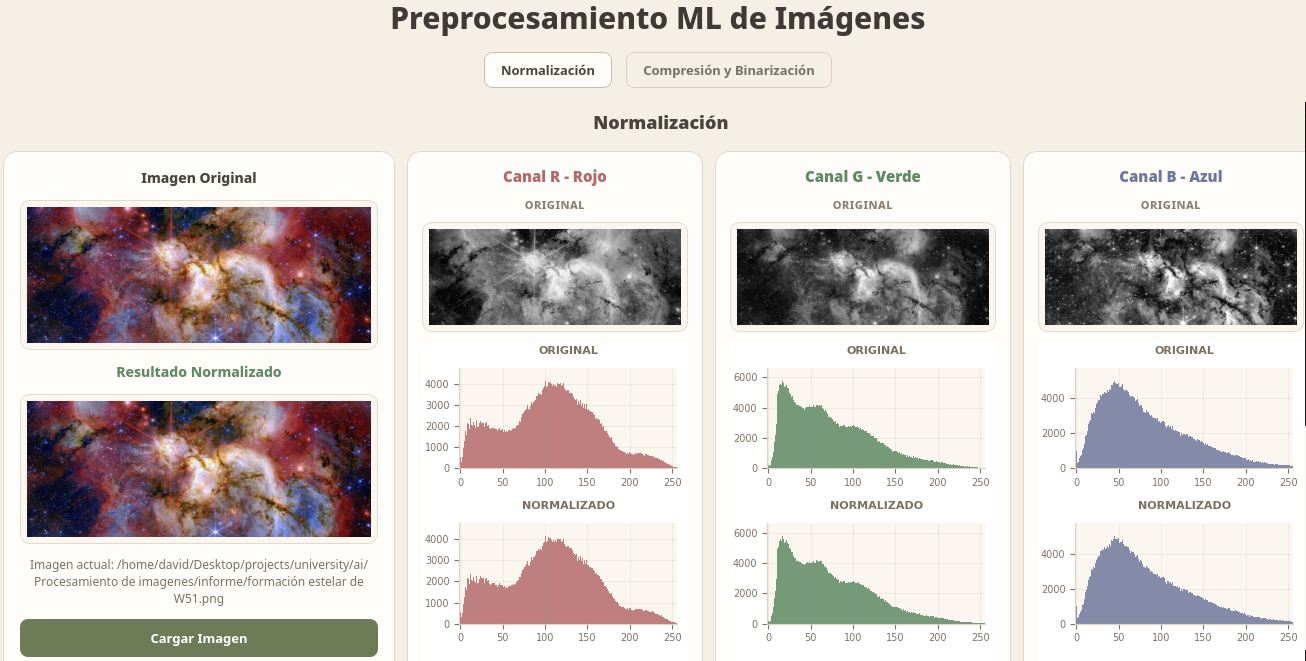
\includegraphics[width=0.92\textwidth]{img/app_interfaz_w51.png}
    \caption{Vista general de la herramienta durante una ejecución de prueba.}
    \label{fig:app_interfaz}
    \vspace{2pt}
    {\footnotesize Fuente: Elaboración propia.}
\end{figure}

\subsection{Resultados obtenidos}

En esta etapa se siguió un flujo fijo que parte desde una sola imagen de entrada y genera una base binaria común para las dos ramas principales del proyecto.

\subsubsection{Preprocesamiento}

La conversión a escala de grises aplica la fórmula de luminosidad ponderada:
\begin{equation}
    I_{gris} = 0.299 \cdot R + 0.587 \cdot G + 0.114 \cdot B
    \label{eq:grises}
\end{equation}
Después se aplica una ecualización manual del histograma para redistribuir las intensidades de la imagen en grises y mejorar el contraste global. Sobre esta imagen ecualizada se define un umbral $T$ para producir una imagen binaria:
\begin{equation}
    I_{bin}(x,y)=
    \begin{cases}
        255, & \text{si } I(x,y)\geq T \\
        0, & \text{si } I(x,y)<T
    \end{cases}
    \label{eq:binaria}
\end{equation}

Finalmente se agrega ruido sal y pimienta. Esta salida se usa como base compartida para comparar de manera justa el dominio espacial y el dominio de frecuencia.

\subsubsection{Resultados en dominio espacial}

En el dominio espacial se implementaron tres filtros manuales: media, mediana y moda. Los tres recorren vecindades cuadradas de tamaño impar y generan una nueva imagen a partir de la información local de cada píxel.

\begin{itemize}
    \item \textbf{Media:} promedia los valores de la ventana y suaviza la imagen.
    \item \textbf{Mediana:} ordena los valores de la ventana y toma el valor central, siendo especialmente útil frente al ruido sal y pimienta.
    \item \textbf{Moda:} selecciona el valor más repetido de la ventana, por lo que se comporta bien cuando la imagen es binaria.
\end{itemize}

Además, la interfaz muestra un mapa de cambio, calculado como diferencia absoluta entre la imagen con ruido y la imagen filtrada. Este recurso permite ver en qué zonas actuó con mayor intensidad el filtro seleccionado.

\subsubsection{Resultados en dominio de frecuencia}

En el dominio de frecuencia se aplica un filtro gaussiano pasa bajas. Para lograrlo se utiliza la FFT (\textit{Fast Fourier Transform}), que es un algoritmo eficiente para calcular la transformada discreta de Fourier. Su función es llevar la imagen desde el dominio espacial al dominio de frecuencia, donde la información puede analizarse en términos de componentes lentas y rápidas.

En imágenes, las bajas frecuencias están asociadas a variaciones suaves de intensidad y las altas frecuencias a detalles finos, bordes y parte del ruido. Una vez calculado el espectro, se construye manualmente la máscara gaussiana:
\begin{equation}
    H(u,v)=e^{-D(u,v)^2/(2D_0^2)}
    \label{eq:gauss}
\end{equation}
donde $D(u,v)$ es la distancia al centro del espectro y $D_0$ controla qué tan amplio es el paso de bajas frecuencias.

La máscara se multiplica punto a punto por el espectro y luego se aplica la transformada inversa para reconstruir la imagen filtrada. La interfaz presenta tres vistas de apoyo: el espectro FFT, la máscara gaussiana y la imagen reconstruida.

\subsubsection{Resumen del flujo implementado}

El flujo real del proyecto puede resumirse así:
\begin{center}
RGB $\rightarrow$ grises $\rightarrow$ ecualización $\rightarrow$ binarización $\rightarrow$ ruido
\end{center}
\begin{center}
base con ruido $\rightarrow$ filtro espacial \hspace{1cm} base con ruido $\rightarrow$ FFT $\rightarrow$ filtro gaussiano
\end{center}

Este diseño permite comparar dos enfoques distintos partiendo exactamente de la misma imagen alterada por ruido.

\subsection{Habilidades blandas empleadas en la práctica}
$\blacksquare$ Trabajo en equipo \\
$\blacksquare$ Responsabilidad \\
$\blacksquare$ Pensamiento crítico

\subsection{Conclusiones}

La aplicación desarrollada permitió construir un flujo completo de procesamiento que inicia en una imagen RGB, pasa por una etapa de preprocesamiento manual y culmina en una comparación entre filtros espaciales y filtrado en frecuencia. El resultado principal del trabajo es que ambos enfoques pueden analizarse sobre una misma base binaria con ruido, lo que facilita una comparación visual directa.

Los filtros espaciales de media, mediana y moda fueron implementados manualmente, lo que permitió comprender con mayor detalle cómo opera cada vecindad sobre la imagen. Entre ellos, mediana y moda resultan especialmente adecuados cuando la entrada es binaria y contiene ruido sal y pimienta.

El filtro gaussiano pasa bajas en frecuencia mostró una lógica distinta: en lugar de trabajar directamente sobre píxeles vecinos, actúa sobre el espectro de la imagen usando la FFT y una máscara construida en el código. Esta diferencia permitió reforzar la comprensión entre procesamiento local en el espacio y procesamiento espectral en frecuencia.

\subsection{Recomendaciones}

Se recomienda trabajar con imágenes de tamaño moderado cuando se utilicen máscaras espaciales grandes, ya que los filtros manuales incrementan su costo computacional conforme aumenta la resolución.

También se recomienda ajustar con cuidado el umbral de binarización, la cantidad de ruido, el tamaño de la máscara y el parámetro $D_0$, porque cada uno afecta de manera visible el resultado final y la comparación entre métodos.

Como mejora futura puede incorporarse una versión optimizada del procesamiento para pruebas rápidas, manteniendo una versión manual como referencia académica para explicar el algoritmo.

\subsection{Referencias bibliográficas}
{
    \renewcommand{\refname}{}
    \vspace{-1.5em}

    \begin{thebibliography}{99}
        \bibitem{gonzalez}
        R. C. Gonzalez and R. E. Woods, \textit{Digital Image Processing}, 4th ed. New York, NY, USA: Pearson, 2018.

        \bibitem{jain}
        A. K. Jain, \textit{Fundamentals of Digital Image Processing}. Englewood Cliffs, NJ, USA: Prentice Hall, 1989.

        \bibitem{szeliski}
        R. Szeliski, \textit{Computer Vision: Algorithms and Applications}, 2nd ed. Cham, Switzerland: Springer, 2022.
    \end{thebibliography}
}

\end{document}
